\chapter{Background to the Jordan Curve Theorem for Polygons}\label{chapter:JordanInformal}
THEOREM~9 in the 10th edition of the \emph{Grundlagen der Geometrie} is the focus of this thesis. It may only be a special case of the full Jordan Curve Theorem, but in the setting of ordered geometry, it is quite involved. In this brief chapter, we will draw together a number of historical threads and characters connected to the theorem and the \emph{Grundlagen der Geometrie}, and we will look at the first published proof attempt by Veblen. This proof is severely inadequate, but there is enough to salvage from the approach to give a correct proof whose verification we leave to Chapters~\ref{chapter:JordanVerification1} and \ref{chapter:JordanVerification2}.

\section{Relationship with the Full Jordan Curve Theorem}\label{sec:JordanCurveHistory}
The full Jordan Curve Theorem effectively says that, when it comes to closed curves that do not self-intersect (\emph{simple closed curves}), we are justified in our use of the expressions ``inside the curve'' and ``outside the curve''. The idea that mathematicians should even bother justifying this appears relatively late in the history of mathematics. In fact, it had to wait until the 19th century and the rigorous reformulations of analysis which reduced the unclear notions governing the continuum to precisely defined formulas involving the now standard $\epsilon$ and $\delta$ inequalities. Bolzano, who is credited along with Cauchy for spotting the reformulation, provided his own rigorous definitions for closed, continuous curves and what it means for curves to enclose points, so that he was then able to recommend the following for rigorous proof:

\begin{quote}
  ``If a closed line lies in a plane and if by means of a connected line one joins a point of the plane which is enclosed within the closed line with a point of the plane which is not enclosed within it, then the connected line must cut the closed line.''
  \flushright{\cite[p. 285]{BolzanoJordan}}
\end{quote}

This is a significant half of the Jordan Curve Theorem, and, reading the terms ``closed lines'' intuitively, it seems so blindingly obvious that one might think it perverse to demand a proof. However, the rigorous definitions which Bolzano had in mind to replace ``closed line'' are not so immediately intuitive, but appeal to very general and abstract topological properties. The first proof that these abstract properties preserve intuitive properties such as Bolzano's conjecture was given in Jordan's 1887 \emph{Cours d'analyse}~\cite{JordanTextBook}. To this day, the proof is regarded as challenging, and one possible reason for the complexity is that the rigorous formulations are so general that they admit weird pathologies, or as Poincar\'{e} colourfully called them, \emph{monsters}. Some of these monsters, such as closed curves enclosing finite area but having infinite length, immediately thwart a number of obvious proof strategies.

Relevant to this chapter is the case against Jordan's proof: common folklore says that it is invalid, and that the first correct proof was provided by Veblen in 1905~\cite{VeblenJordan}. Both Veblen and folklore point out that Jordan had to assume the polygonal case, and argue that he should have proven this as a lemma. Hales, on the other hand, has formally verified the theorem in HOL~Light, and put together a strong defence of Jordan~\cite{HalesJordansProof}, and of a basically elegant and correct proof that has been unfairly neglected. The polygonal case is supposedly completely trivial. 

Not so, according to Feferman. In his paper concerning the aforementioned \emph{monsters}~\cite{FefermanDevilishJCT}, he repeats the folklore that Veblen gave the first correct proof, and claims that even the polygonal case is ``devilishly difficult to prove.''

There is already controversy with Hilbert's 1899 edition of the \emph{Grundlagen der Geometrie}. There, Hilbert gave a formulation of the polygonal case as THEOREM~6, but, as with the five preceding theorems, he did not give a proof. Instead, he assures us that with the aid of his theorem for the existence of half-planes (THEOREM~5 of that edition), one can obtain the proof ``without much difficulty.'' This certainly backs up the idea that the theorem is trivial. However, by the Ninth Edition, the clause had been deleted, with the edit noted as a ``correction.'' The theorem still appears without proof, though Bernays, in a supplement to the main text, cites a detailed proof by Fiegl~\cite{FeiglJordan}. Note that Bernays does not \emph{include} the proof, as he does in other cases, such as proving that Pasch's axiom can be rendered without the inclusive-or~(see \S\ref{sec:PaschInclusiveOr}). That would have taken more than a few supplementary remarks.

Now Veblen, one year before publishing his proof of the Jordan Curve Theorem, had developed an axiomatic foundation for geometry which was very close to Hilbert's own~\cite{Veblenphd}, and in his thesis, he expends a great deal more effort developing a theory of order than did Hilbert. This explains why Veblen's doctoral supervisor, E.~H.~Moore, was contributing proofs to later editions of Hilbert's text~(see \S\ref{sec:Theorem5}). It also explains why, in Veblen's 1905 proof of the full Jordan Curve Theorem, he thought it necessary to cite a proof from his doctoral thesis showing that the Jordan Curve Theorem holds for the even more trivial case of \emph{triangles}. Plausibly, Veblen's criticism of Jordan can be explained by his particular standards of rigour and the context of an axiomatic theory of geometry. 

Another aspect we should consider is the level of generality that Veblen was attempting. He gave a proof of the full theorem in the context of ordered geometry with the addition of one topological axiom. As such, the proof was not supposed to require any assumptions about the existence of a metric. Unfortunately, as Hales points out in his defence of Jordan~\cite{HalesJordansProof}, such generality was refuted ten years later by R. L. Moore\footnote{Not to be confused with Veblen's supervisor E.~H.~Moore.}, who had been a student of Veblen's. %before he turned to evil
Moore showed that in Veblen's setting, all planes are homeomorphic to the Euclidean plane~\cite{MooreSitus}, and thus his axioms always describe a metrisable space.

But what about the polygonal case? In his doctoral thesis, Veblen gave a detailed, standalone proof of this theorem without using the topological axiom. The theorem, then, is plausibly still very general. So one question is: given its generality, is it still \emph{trivial}? We suggest not. As we discuss in \S\ref{sec:VeblenProof}, a correct proof seems to have eluded Veblen himself.

\section{Generality of the Polygonal Case}\label{sec:JordanCurveGenerality}
We can discuss the generality of ordered geometry by considering the two proofs of the polygonal theorem from the book \emph{What Is Mathematics?}~\cite{WhatIsMathematics}. Hales mentions these to highlight the triviality of the polygonal case. The first of the proofs is the so-called ``plumb-line'' proof. We begin with a simple polygon, pick an arbitrary direction which is not parallel to any of its sides, and then for any point, we cast a ray in that direction. By considering the number of times the ray crosses the polygon, and how this number changes as we move around the plane, we can prove the polygonal case.

This is a non-starter. The notion of \emph{direction} should either be formalised in terms of angles, giving a compass direction, or in terms of equivalence classes of parallel lines. In Group~II, we cannot say that parallel lines even \emph{exist}. This matter is settled in Group~IV, where the parallel axiom appears. Theorems for angle construction and congruence are also unavailable, based on axioms only available in Group~III. We also have no formulations of what it means to ``move'' along a ray. The sort of motion being considered is presumably \emph{continuous} motion, and indeed, if we look at Tverberg's proof of the theorem~\cite{TverbergJordan}, he essentially gives the same argument in rigorous form, and appeals directly to continuity. But  continuity does not appear in Hilbert's text until Group~V. 

The second proof from \emph{What Is Mathematics?} only states an approach, and does not provide a complete proof. It effectively says we can prove the Jordan Curve Theorem for polygons by computing winding numbers for the polygon. A na\"{i}ve formulation of this argument in terms of angles and continuous motion will be well outside the scope of Hilbert's first two groups of axioms, for the same reasons as above. 

To reiterate, the problem we have with traditional proofs of the Polygonal Jordan Curve Theorem is that our axioms are too weak to formulate them. Another way to put this is to say that the version of the theorem we are attempting to prove is more general than the traditional versions, and must apply to \emph{any} ordered geometry. A visual way to bring this point home is to note that by ``simple polygons'', we are actually including the boundaries of all possible \emph{mazes} which do not contain loops, such as the one shown in Figure~\ref{fig:SimplePolygon}. Moreover, we are allowing the corridors of these mazes to be infinitesimally narrow, since we do not rule out non-Archimedean geometries at this stage.

Furthermore, we are tasked with navigating these mazes without being able to measure any distances. We cannot orient ourselves, rotate or compare directions. We cannot consider continuous motion. And we know nothing about the existence of parallel lines. In other words, we are navigating without a ruler, without a compass, and without being able to run a path parallel to a wall. We suspect these constraints will eliminate most trivial proofs.

\begin{figure}
\centering
\includegraphics[scale=0.4]{jordan/denseMaze.pdf}
\caption{A simple polygon}
\label{fig:SimplePolygon}
\end{figure}

\section{Polygonal Case: Formulation}\label{sec:JordanCurveExplanation}
The full Jordan Curve theorem applies to arbitrary simple closed curves, and characterises the interior and exterior in terms of path-connectedness. The polygonal version of the Jordan Curve Theorem replaces ``simple closed curve'' with ``simple polygon'', and characterises the two regions in terms of \emph{polygonal}-path connectedness. That is, the interior and exterior of the polygon are the largest sets all of whose points can be joined by polygonal paths. 

The three primitives at Hilbert's disposal, namely two incidence relations and a betweenness relation, are sufficient to formulate the notion of polygons, interiors and exteriors. Having already defined a segment as an unordered pair of points, Hilbert defines a \emph{polygonal segment}\footnote{Veblen calls these \emph{broken lines}.} as follows:

\begin{quotation}
  DEFINITION. A set of segments $AB$, $BC$, $CD$, $\ldots$, $KL$ is called a \emph{polygonal segment} that connects the points $A$ and $L$. Such a polygonal segment will also be briefly denoted by $ABCD\ldots KL$. The points inside the segments $AB$, $BC$, $CD$, $\ldots$, $KL$ as well as the points $A$, $B$, $C$, $D$, $\ldots$, $K$, $L$ are collectively called the \emph{points of the polygonal segment}.
  \flushright{\cite[p. 8]{FoundationsOfGeometry}}
\end{quotation}

Polygons are then polygonal segments where the points $A$ and $L$ coincide. For polygons, we refer to each of the individual segments $AB$, $BC$, $\ldots$, $KL$ as a \emph{side} of the polygon. Finally, Hilbert defines \emph{simple polygons}:

\begin{quote}
  ``If the vertices of a polygon are all distinct, none of them falls on a side and no two of its nonadjacent sides have a point in common, the polygon is called \emph{simple}.''
  \flushright{\cite[p. 9]{FoundationsOfGeometry}}
\end{quote}

Like the rays and half-plane theorems, the Polygonal Jordan Curve Theorem describes a partitioning of a space into two ``connected'' regions, where connectedness is cashed out in terms of a suitable relation. Here, we are told that the polygon partitions all other points in the plane as follows:

\begin{quotation}
  THEOREM 9. Every single polygon lying in a plane $\alpha$ separates the points of the plane $\alpha$ that are not on the polygonal segment of the polygon into two regions, the \emph{interior} and the \emph{exterior}, with the following property: If $A$ is a point of the interior {\bfseries (an interior point)} and $B$ is a point of the exterior {\bfseries (an exterior point)} then every polygonal segment that lies in $\alpha$ and joins $A$ with $B$ has at least one point in common with the polygon. On the other hand if $A$, $A'$ are two points of the interior and $B$, $B'$ are two points of the exterior then there exist polygonal segments in $\alpha$ which join $A$ with $A'$ and others which join $B$ with $B'$, none of which have any point in common with the polygon. By suitable labelling of the two regions there exist lines in $\alpha$ that always lie entirely in the exterior of the polygon. However, there are no lines that lie entirely in the interior of the polygon.

  \centering\includegraphics[scale=0.8]{jordan/jordanHilbert.pdf}
\flushright{\cite[p. 9]{FoundationsOfGeometry}}
\end{quotation}

% \section{Point-in-Polygon Proof}\label{sec:JordanCurveFirstProof}
% One feature of Veblen's proof, and the proof we verify in Chapter~\ref{chapter:JordanVerification1}, is that the treatment of the two regions defined by a simple polygon is symmetric. This means, however, that unlike the plumb-line and winding number proofs from \emph{What is Mathematics?}, Veblen's proof does not hint at any sort of point-in-polygon \emph{test}, one that could be implemented on a machine.

% Before we encountered Veblen's proof, we had developed one of our own which does allow for such a test, by reducing the problem of deciding whether a point is inside a polygon to the problem of deciding whether a point is on a given side of each of the polygon's diagonals. The proof is inductive over the vertices of a simple polygon, and goes some way towards thinking of the Jordan Curve Theorem for polygons as a triangulation problem.

% We decided to try an inductive proof on the total number of vertices of a simple polygon. To do this, it is necessary to show that every simple polygon can be broken down into smaller, simple polygons, until one reaches the smallest possible polygon (the triangle). We have verified the Polygonal Jordan Curve Theorem in this base case as part of our main verification in Chapters~\ref{chapter:JordanVerification1} and~\ref{chapter:JordanVerification2}.

% The idea that we might be triangulating polygons in this proof should give us pause, once we realise that most proofs that a polygon can be triangulated assume the Jordan Curve Theorem for polygons~\cite{PolygonsHaveEars}. We are thus in danger of creating a circular argument. We avoid this danger because firstly, at each stage, we do not require that the smaller polygons are subsets of the original (thus, we do not actually identify a triangulation). And secondly, we are always able to use the Polygonal Jordan Curve Theorem as an inductive hypothesis at each stage.

% Now to split a given simple $n$-gon where $n>3$ into two simple polygons, we just pick a line connecting two non-adjacent vertices, a \emph{diagonal}, which does not intersect the polygon. The simplest example of interest is the concave quadrilateral shown in Figure~\ref{fig:quadConcave}. This quadrilateral has exactly two diagonals. The diagonal $P_2P_4$ lies in the interior of the polygon, while the diagonal $P_1P_3$ lies in the exterior.

% \begin{figure}
%   \centering
%   \includegraphics[scale=0.8]{jordan/quadConcave.pdf}
%   \caption{Concave Quadrilateral}
%   \label{fig:quadConcave}
% \end{figure}

% If we take the diagonal $P_2P_4$, we see that the interior of the quadrilateral consists of the union of the interiors of two triangles, namely $P_1P_2P_4$ and $P_2P_3P_4$, together with the diagonal $P_2P_4$ itself (see Figure~\ref{fig:quadUnion}). If we take the diagonal $P_2P_4$, then we see the interior of the quadrilateral consists of the interior of the triangle $P_1P_3P_4$, minus the interior of $P_1P_2P_3$ and the boundary of $P_1P_2P_3$. Thus, we can always define the interior of the quadrilateral in terms of the interiors of two triangles arising from a diagonal. We shall extend this to the general case for an $n$-gon with $n>3$.

% \begin{figure}
%   \centering 
%   \subfigure[Union of Two Triangles]{\includegraphics[scale=0.8]{jordan/quadUnion1.pdf}
%     \includegraphics[scale=0.8]{jordan/quadUnion2.pdf}
%     \includegraphics[scale=0.8]{jordan/quadUnion3.pdf}
%     \label{fig:quadUnion}}

%   \subfigure[Difference of Two Triangles]{\includegraphics[scale=0.8]{jordan/quadDiff1.pdf}
%     \includegraphics[scale=0.8]{jordan/quadDiff2.pdf}
%     \includegraphics[scale=0.8]{jordan/quadDiff3.pdf}
%     \label{fig:quadDiff}}
%   \caption{Decomposing a Concave Quadrilateral}
%   \label{fig:quadDecompose}
% \end{figure}

% The rest of this section contains all the core ideas of the proof. The proof has not been verified, but we consider it an interesting contribution in its own right. It is distinguished from the proof we \emph{have} verified since it yields a very simple point-in-polygon test by recursively subdividing a polygon and ultimately reducing the problem to point-in-triangle tests.

% The following subsections are quite dense, and details of the proof may not be convincing on a first read. We ask the reader to take the matter on trust. With our experience verifying the Polygonal Jordan Curve Theorem and with our hindsight, we are very confident that the proof is correct and can be verified by reusing much of the verification discussed in Chapters~\ref{chapter:JordanVerification1} and~\ref{chapter:JordanVerification2}. A full verification makes for suitable further work. 

% \subsection{Finding a Diagonal}\label{sec:FindingDiagonal}
% A simple polygon $P_1P_2 \ldots P_n$ where $n>3$ has at least one diagonal which does not intersect the polygon. To see this, we assume without loss of generality that $P_1P_2P_3$ are non-collinear. Consider the line $P_1P_3$. If this line does not intersect the polygon, then it is a suitable diagonal. Otherwise, take the vertex $P_m$ where $3 < m < n$ such that the line $P_1P_m$ intersects $P_2P_3$ in a point $X$ and such that, for any other $P_{m'}$ where $3 < m' < n$, if $P_1P_{m'}$ intersects $P_2P_3$ at $X'$, then $X$ is between $P_1$ and $X'$. We then have that $P_1P_m$ is the required diagonal, which yields two smaller simple polygons, shown in green and blue (see Figure~\ref{fig:SqueezeDemo}).

% A \emph{very} slightly modified version of this argument is a core component in the proof we actually verified. We shall explain it in more detail in \S\ref{sec:Squeeze}.

% \begin{figure}
% \centering
% \includegraphics{jordan/diagonal.pdf}
% \caption{Finding a Diagonal}
% \label{fig:SqueezeDemo}
% \end{figure}

% \subsection{Cases}
% As noted, a diagonal $D$ of a polygon $p$ that does not intersect $p$ divides it into two smaller polygons $p_1$ and $p_2$. Generalising the situation from Figure~\ref{fig:quadDecompose}, we have that if $D$ is interior to $p$, then the interior of $D$ can be defined as the union of the interiors of $p_1$ and $p_2$, together with $D$. On the other hand, if $D$ is exterior to $p$, and the interior of $p_2$ is a subset of the interior of $p_1$, then we can define, without loss-of-generality, the interior of $p$ to be the interior of $p_1$ minus the boundary and interior of $p_2$. It therefore follows that the interior of a polygon is formed by recursively adding and subtracting out the interiors of smaller polygons. Finally, at each step, we define the exterior of the polygon as the plane minus the interior and minus the polygon's boundary.

% There is obviously circularity here, since whether or not $D$ is an interior or exterior diagonal should be a \emph{corollary} of our argument. To remedy this, we shall need to characterise the two cases some other way.

% In Figure~\ref{fig:DiagonalCases}, we illustrate the two cases by showing a fragment of a polygon and its diagonal. Here, we assume that the polygon $p$ is of the form $P$, $P_1$, $P_2$, $P_3$, $P_4$, $P_5$, $Q$, $Q_1$, $Q_2$, $Q_3$, $Q_4$, $Q_5$ and has a diagonal $PQ$ which does not intersect $p$. Our recursive step involves splitting the polygon into $p_1 = P, P_1, P_2, P_3, P_4, P_5, Q$ and $p_2 = Q, Q_1, Q_2, Q_3, Q_4, Q_5, P.$

% We now take a point $X$ on the diagonal $PQ$, and we cast rays out to the points $Y$ and $Z$ on either side of $PQ$, such that $X$ is the only point of intersection of the segment $YZ$ and the polygons $p_1$ and $p_2$ (ray-casting will be discussed in \S\ref{sec:RayCasting}). 

% We now make the following inductive hypotheses:
% \begin{description}\label{sec:FirstProofInductiveHypotheses}
% \item[IH1] Interior points $A$ and $B$ of $p_1$ can be connected by a polygonal path which does not intersect $p_1$, and similarly for $p_2$.
% \item[IH2] Exterior points $A$ and $B$ of $p_1$ can be connected by a polygonal path which does not intersect $p_1$, and similarly for $p_2$.
% \item[IH3] Any path connecting an interior point $A$ of $p_1$ to an exterior point $B$ of $p_1$ must intersect $p_1$, and similarly for $p_2$.
% \item[IH4] If $Y'$ and $Z'$ are endpoints of a segment which crosses exactly one side of $p_1$, then they lie in different regions with respect to $p_1$ (and similarly for $p_2$).
% \item[IH5] If another segment $Y'Z'$ does not intersect any side of $p_1$, nor any side of $p_2$, then $Y'$ and $Z'$ lie in the same region.
% \end{description}

% Assuming that interiors and exteriors are non-empty and cover the plane, the first three hypotheses are equivalent to the polygonal Jordan Curve Theorem. 

% IH4 gives us the following two cases:
% \begin{enumerate}
% \item The point $Y$ lies in the interior of one of $p_1$ or $p_2$ and $Z$ lies in the interior of the other (see Figure~\ref{fig:UnionCase}).
% \item One of $Y$ and $Z$ lies in the exterior of both $p_1$ and $p_2$ (see Figure~\ref{fig:SubCase}).
% \end{enumerate}

% The first case corresponds to $PQ$ being an interior diagonal. The second case corresponds to $PQ$ being an exterior diagonal.

% \begin{figure}
% \centering
% \subfigure[Union for Interior Diagonal]{\includegraphics[scale=0.9]{jordan/unionCase.pdf}
%   \label{fig:UnionCase}}
% \subfigure[Subtraction for Exterior Diagonal]{\includegraphics[scale=0.9]{jordan/diffCase.pdf}
%   \label{fig:SubCase}}
% \caption{Diagonal Cases}
% \label{fig:DiagonalCases}
% \end{figure}

% \begin{figure}
% \centering
% 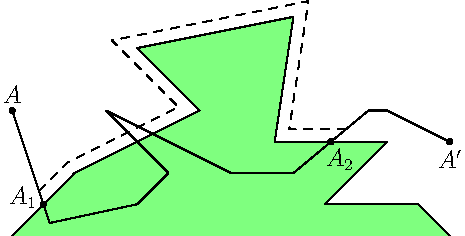
\includegraphics{jordan/navigation1.pdf}
% \caption{Navigating around the Exterior}
% \label{fig:Navigation1}
% \end{figure}

% \begin{figure}
% \centering
% \subfigure[Union Case]{\includegraphics[scale=0.9]{jordan/shorten1.pdf}\label{fig:Shorten1}}
% \subfigure[Subtraction Case]{\includegraphics[scale=0.9]{jordan/shorten2.pdf}\label{fig:Shorten2}}
% \caption{Paths for IH3}
% \end{figure}

% \subsection{Union Case}
% For the case depicted in Figure~\ref{fig:UnionCase}, we will assume, without loss of generality, that $Y$ lies in the interior of $p_1$ and $Z$ lies in the interior of $p_2$. Since $YZ$ crosses $PQ$, we know from IH4 that $Y$ is exterior to $p_2$ and $Z$ exterior to $p_1$, and by IH1 and IH5, we know further that all interior points of $p_1$ are exterior to $p_2$ and all interior points of $p_2$ are exterior to $p_1$.

% We now define the interior of $p$ as the union of the interiors of $p_1$ and $p_2$ and the interior of the diagonal $PQ$. We define the exterior as the set of points not on the polygon and not in the interior. We just need to reprove IH1--IH5 as IH$'$--IH5$'$ for the polygon $p$.

% \begin{description}
% \item[IH{1}$'$] Interior points $A$ and $B$ of $p$ can be connected by a polygonal path which does not intersect~$p$.
%   \begin{proof}
%     Suppose $A$ and $B$ both lie inside $p_1$, or both lie inside $p_2$. We apply IH1 to $p_1$ and $p_2$, and thereby connect $A$ and $B$ with a polygonal segment lying in the interior of $p$. On the other hand, if we suppose (without-loss-of-generality) that $A$ is inside $p_1$ and $B$ is inside $p_2$, then we apply IH1 to $p_1$ in order to connect $A$ to $Y$, and we apply IH1 to $p_2$ in order to connect $B$ to $Z$. The required path can then be completed with the segment $YZ$.
%   \end{proof}
% \item[IH{2}$'$] Exterior points $A$ and $B$ of $p$ can be connected by a polygonal path which does not intersect $p$.
%   \begin{proof}
%     We must have that $A$ and $B$ lie in the exteriors of both $p_1$ and $p_2$. By IH2 applied to $p_1$, there is a path through the exterior of $p_1$ which connects $A$ and $B$. If this path lies entirely in the exterior of $p_2$ then it also lies entirely in the exterior of $p$ and we are done. 

%     Otherwise, by IH3, there must be a first point $A_1$ and a last point $A_2$ at which the path crosses the boundary of $p_2$. By IH5, the path from $A$ to $A_1$ and the path from $A_2$ to $B$ must lie in the exterior of $p_2$. We then find a new path which follows the edges of the polygon until it connects these two points. This path then lies in the exterior of $p_2$ and so in the exterior of $p$. See Figure~\ref{fig:Navigation1} for an illustration and see \S\ref{sec:Jordan1NavigationDiscussion} for some discussion on this part of the proof.
%   \end{proof}
% \item[IH{3}$'$] Any path connecting an interior point $A$ of $p$ to an exterior point $B$ of $p$, must intersect $p$.
%   \begin{proof}
%     Assume, without loss-of-generality, that $A$ lies in the interior of $p_1$ and $B$ lies in the exterior of both $p_1$ and $p_2$, and consider any polygonal path connecting $A$ and $B$. Since $B$ lies in the exterior of $p_1$, the path must intersect $p_1$ by IH3. If it intersects any side of the polygon $p_1$ other than $PQ$, we are done.

% Otherwise, suppose the path intersects $PQ$ as in Figure~\ref{fig:Shorten1}, and take the last such point of intersection $R$ as we move towards $B$. We then consider a point $A'$ just beyond $R$ such that $A'Z$ does not intersect $p_2$ and is therefore in the interior of $p_2$ by IH5 (see \S\ref{sec:Jordan1SameSideDiscussion} for some discussion). The subpath from $A'$ to $B$ now connects a point interior to $p_2$ to a point exterior to $p_2$ which does not cross $PQ$. Hence, by IH3, the subpath must intersect $p_2 - PQ$ at a point $S$. This point $S$ must be a point on~$p$.
%   \end{proof}
% \item[IH{4}$'$] If $Y'$ and $Z'$ are endpoints of a segment which crosses exactly one side of $p$, then one point is interior while the other is exterior with respect to $p$.
%   \begin{proof}
%     Suppose $Y'Z'$ crosses a side of $p$. Without loss-of-generality, we can assume that this is a side of $p_1$ other than $PQ$, and then apply IH4. This tells us that $Y'$ and $Z'$ lie in opposite regions with respect to $p_1$, and so one of the points, say $Y'$ lies inside $p_1$, while $Z'$ lies outside $p_1$.

%     But the fact that $Y'$ is inside $p_1$ means that it must be outside $p_2$, and because $Y'Z'$ does not intersect $p_2$ (since $p$ is simple), we know from IH5 that $Z'$ also lies outside $p_2$. Thus, $Z'$ lies outside $p$, as required.
    
%   \end{proof}
% \item[IH{5}$'$] If a segment $Y'Z'$ does not intersect $p$, then $Y'$ and $Z'$ lie in the same region.
%   \begin{proof}
%     If the segment does not intersect any side of $p$ and does not intersect any sides of $p_1$ or $p_2$, then the case reduces to IH5 applied to $p_1$ and $p_2$. If it does intersect $p_1$ or $p_2$, then the side intersected must be the diagonal $PQ$. In this case, we can find a path which does not intersect $p_1$ and which connects $Y$ to $Y'$, or a path which does not intersect $p_2$ and which connects $Y$ to $Z'$. Thus, $Y'$ is interior to one of $p_1$ and $p_2$ by IH5 and thus interior to $p$. The same argument applies to $Z'$. See \S\ref{sec:Jordan1SameSideDiscussion} for some further discussion. % Note that the above disjunction is a case-split on which side of $PQ$ the points $Y'$ and $Z'$ are on. I am confident that the step corresponds exactly to the use of same_side_wall_connected in the verified proof.
%   \end{proof}
% \end{description}

% \subsection{Subtraction Case}
% The second case differs from the first in that we lose the symmetry between $p_1$ and $p_2$. One of the polygon's interior must be contained entirely by the other's.

% We can determine which by considering whether $P_1$ lies inside $p_2$ or whether $Q_1$ lies inside $p_1$. To see why these are alternatives, suppose that $P_1$ does not lie inside $p_2$ (as depicted in Figure~\ref{fig:SubCase}). Then it follows from IH5 and the fact that $p$ is simple that $p_1 - PQ$ lies outside $p_2$. 

% We then consider a path between $Z$ and $Q_1$ whose interior does not intersect $p_2$ (see \S\ref{sec:Jordan1SameSideDiscussion} for discussion). Since the interior of this path lies inside $p_2$, while the path $p_1 - PQ$ lies outside $p_2$, it follows that the path does not intersect $p_1$. Hence, by IH5, $Q_1$ lies with the point $Z$, inside $p_1$.

% We have thus shown that either $P_1$ lies inside $p_2$ or $Q_1$ lies inside $p_1$. Now assume, without loss of generality, that $Q_1$ is interior to $p_1$ as depicted in Figure~\ref{fig:SubCase}. In this case, all points interior to $p_2$ are also interior to $p_1$. Indeed, by IH1, any interior point $A$ of $p_2$ can be connected to $Z$ by a path which does not interspect $p_2$, and which therefore, by IH5, lies entirely in the interior of $p_2$. Since $p_1 - PQ$ lies exterior to $p_2$, we know that the path does not intersect $p_1$, and so again by IH5, we know that the path lies entirely in the interior of $p_1$. We thus know that its endpoint $A$ lies in the interior of $p_1$.

% We now prove IH1$'$--IH5$'$ for the step case.

% \begin{description}
% \item[IH1$'$] Interior points $A$ and $B$ of $p$ can be connected by a polygonal path which does not intersect~$p$.
%   \begin{proof}
%     An interior point of $p$ is an interior point of $p_1$ which is not interior to $p_2$. If we apply IH1 to $p_1$, we can find a path between $A$ and $B$ through the interior of $p_1$. It is possible that this path intersects $p_2$, and so we must appeal to the same argument used for IH2$'$ in the union case and depicted in Figure~\ref{fig:Navigation1}, in order to navigate through the exterior of $p_2$.
%   \end{proof}
% \item[IH2$'$] Exterior points $A$ and $B$ of $p$ can be connected by a polygonal path which does not intersect $p$.
%   \begin{proof}
%     This argument is similar to that given for IH1$'$ in the union case. If both $A$ and $B$ lie in the exterior of $p_1$, then we know from IH1 applied to $p_1$ that they can be connected by a path exterior to $p_1$. And since $p_2 - PQ$ is interior to $p_1$ by IH5, we know that this path does not intersect $p$.

%     Similarly, if $A$ and $B$ lie in the interior of $p_2$, we know from IH1 that they can be connected by a path interior to $p_2$. And since $p_1 - PQ$ is exterior to $p_2$, we know that this path does not intersect $p$.

%     Finally, if we assume without-loss-of-generality that $A$ is exterior to $p_1$ and $B$ interior to $p_2$, then we can join $A$ to $Y$ by a path exterior to $p_1$ and thus one which does not intersect $p_2$, and join $B$ to $Z$ by a path interior to $p_2$ and thus one which does not intersect $p_1$. The segment $YZ$ then completes a path connecting $A$ to $B$ which does not intersect $p$.
%     \end{proof}

% \item[IH3$'$] Any path connecting an interior point $A$ of $p$ to an exterior point $B$ of $p$, must intersect $p$.
%   \begin{proof}
%     The proof is similar to that for the previous section. By definition, $A$ lies inside $p_1$ and outside $p_2$. The point $B$, on the other hand, might lie outside $p_1$, inside $p_2$, or it might lie on the diagonal $PQ$. If the path between them does not intersect the diagonal $PQ$, then we know from IH3 that it must intersect some side of $p$ and we are done.

% So let us suppose it intersects the diagonal $PQ$. We now take the first point $R$ on the path from $A$ at which the the diagonal is intersected. Then there will be an earlier point $B'$ on the path which we can connect to $Z$ by a path which does not intersect $PQ$ (see \S\ref{sec:Jordan1SameSideDiscussion} for discussion). Thus, by IH5, $B'$ is either inside $p_2$ or outside $p_1$, and the subpath $AB'$ does not intersect $PQ$. It follows then, applying IH3, that we can find a point $S$ where the subpath intersects $p$. See Figure~\ref{fig:Shorten2} for an illustration.
%   \end{proof}

% \item[IH4$'$] If $Y'$ and $Z'$ are endpoints of a segment which crosses exactly one side of $p$, then they lie in different regions with respect to $p$.
%   \begin{proof}
%      Suppose that $Y'Z'$ intersects a side of $p_1$. If we apply IH4 to $p_1$, we find that one of these points must be interior to $p_1$ and the other exterior. Moreover, since the point of intersection of $Y'Z'$ with $p_1$ is exterior to $p_2$, we can apply IH5 to $p_2$ and conclude that $Y'$ and $Z'$ are both exterior to $p_2$. It follows by the definition of $p$ that $Y'$ and $Z'$ are then in opposite regions. A similar argument applies if $Y'Z'$ intersects a side of $p_2$.
%   \end{proof}
% \item[IH5$'$] If a segment $Y'Z'$ does not intersect $p$, then $Y'$ and $Z'$ lie in the same region.
%   \begin{proof}
%     If $Y'Z'$ does not intersect $p_1$ or $p_2$, then this reduces to the case IH5 applied to these polygons. Otherwise, we suppose that $Y'Z'$ intersects the diagonal $PQ$. 

%     If $Y'$ is inside $p$, then it lies inside $p_1$, and thus $Z'$ must be outside $p_1$ by IH4 applied to $p_1$. Therefore, $Z'$ is outside $p_2$. 

% Moreover, if $Y'$ lies inside $p$, then it too lies outside $p_2$. So the two points lie in the same region with respect to $p_2$. This means we have a contradiction: $Y'Z'$ could not possibly intersect $PQ$ as supposed, for otherwise, they would lie in opposite regions with respect to $p_2$ as required by IH4.

%     Now what if $Y'$ is not inside $p$? Then there are three possibilities for its location:
%     \begin{description}
%     \item[The point $Y'$ lies inside $p_1$ and $p_2$] In this case, we can apply IH4 to $p_1$ and conclude that $Z'$ is outside $p_1$. By definition, both points are then exterior to $p$. 
%     \item[The point $Y'$ lies on $PQ$] In this case, $Z'$ is a point on a ray which is cast from $Y'$ and must therefore lie either in the exterior of $p_1$, in the interior $PQ$ or in the interior of $p_2$. In any case, both $Y'$ and $Z'$ are exterior to $p$.
%     \item[The point $Y'$ lies outside both $p_1$ and $p_2$] Here, we apply IH4 to $p_2$, and thus conclude that the point $Z'$ is inside $p_2$. By definition, both points are then exterior to $p$.
%     \end{description}
%   \end{proof}
% \end{description}

% \subsection{Discussion}
% There are a few definite gaps in this first proof attempt. As said, we neglected to prove the base case for triangles, and we have not shown that the recursively defined interiors and exteriors are always non-empty. We consider these to be fairly straightforward matters, however. 

% This is not the proof we chose to verify, though the one we \emph{have} verified shares many of its inferences. When we come to verify those inferences, we shall see that many details above have been glossed over. We hope, then, to convince the reader to be quite wary of the above proof as it stands. The details that we have glossed over will be put on a more solid footing when we discuss our verification.

% \label{sec:Jordan1NavigationDiscussion}For instance, in Figure~\ref{fig:Navigation1}, we claim to be able to navigate around the exterior of a simple polygon. This intuitive idea will be needed again in our verified proof, where it needs to be carefully formulated, and the formulation needs to be carefully tied back to the premises and the desired conclusion. The details are given in \S\ref{sec:NavigationVerification}.

% \label{sec:Jordan1SameSideDiscussion}At several places in the above proof, we also assumed we could always find a path connecting the points $Y$ and $Z$ in Figures~\ref{fig:UnionCase} and~\ref{fig:SubCase} to various other points. A careful formulation of what characterises such points, together with a proof that the required path can be exhibited, is given in \S\ref{sec:SameSideWallConnected}.

% We have retained the above proof because of its computational properties. It recursively builds the interior of a polygon from the interiors of triangles, and thus describes an algorithm for a point-in-polygon test by reducing the problem to point-in-triangle tests, which, in turn, reduce to point in half-plane tests. Our verified proof does not have this feature. It was inspired by Veblen's proof, and its basic structure and focus are very different. Nevertheless, it is interesting that a number of the key steps overlap, and we shall refer back to this proof when we discuss the verification of the polygonal Jordan Curve Theorem in Chapters~\ref{chapter:JordanVerification1} and~\ref{chapter:JordanVerification2}.

\section{Veblen's Proof}\label{sec:VeblenProof}
In his 1903 doctoral thesis~\cite{Veblenphd}, Veblen set out a basic set of axioms for Euclidean Geometry. His incidence and order axioms are very similar to Hilbert's own, and it should not be difficult to verify their equivalence, but his attention to the elementary theorems of ordered geometry is much more thorough. He proves forty theorems while Hilbert only proves ten, and he attempts a complete proof for the Polygonal Jordan Curve Theorem.

Veblen does not explicitly define the interior or exterior of a polygon. Like most other proofs, he tries to show that the two regions exist implicitly by dividing the result into two claims: the first states that a simple polygon divides its plane into at least two regions; the second states that the polygon divides its plane into at most two regions. Both assertions can be formalised in terms of polygonal segments:
\begin{enumerate}
\item there are at least two points in the plane not on the polygon which cannot be connected by a polygonal segment without crossing the polygon\label{list:VeblenLemma1};
\item of any three points in the plane not on the polygon, at least two of them can be connected by a polygonal segment without crossing the polygon.
\end{enumerate}

Veblen has a two page proof for this and it is one of the most detailed in his thesis, but it is far from persuasive. According to Reeken and Kanovei~\cite{HahnInconclusiveIndirect}, the proof was deemed ``inconclusive'' by Hahn, while Guggenheimer claims, citing Lennes and Hahn, that Veblen's proof assumes that the polygon can be triangulated and is thus only valid for convex polygons~\cite{GuggenheimerJordanCurve}. We could not find this criticism in Lennes~\cite{LennesPolygon}, and indeed, we think Guggenheimer is mistaken here. He may have been misled by the fact that Veblen's proof is based on finding a sequence of triangles whose vertices are shared with the polygon. But this sequence is no \emph{triangulation}. 

We were initially satisfied by Veblen's proof, and so we attempted to verify it. Eventually, as the sceptical Guggenheimer and Hahn might have anticipated, we hit an obstacle, and we had to give up. In the next few sections, we will suggest where Veblen's proof goes wrong.

\subsection{Veblen's Lemma}\label{sec:VeblenLemma1}
The first half of Veblen's proof, showing that there are at least two points not on a polygon which cannot be connected, is given as the corollary to a very general result about polygons. In stating this result, he uses the term ``multiple points'', which are points, should they exist, where a polygon self-intersects:
\begin{quote}
  ``\emph{If a side of a polygon $q$ intersects a side of a polygon $p_n$ in a single point $O$ not a multiple point of $p_n$ or $q$, then $p_n$ and $q$, whether simple or not, have at least one other point in common.}''
  \flushright{\cite[p. 365]{Veblenphd}}
\end{quote}

From this, we can obtain the first half of the Polygonal Jordan Curve Theorem, as we explain in \S\ref{sec:FinalProofJordan1}, but this is already a very general result, and one we draw special attention to when we verify it in Chapter~\ref{chapter:JordanVerification1}. We can see that it holds even for  degenerate polygons. Consider the example in Figure~\ref{fig:jordanDegenerate1}. Here, we have two polygons $P_1P_2P_3$ and $Q_1Q_2Q_3$. The points of these polygons are obviously collinear and so cannot divide the plane into multiple regions. But neither are they a counterexample to Veblen's claim, since their point of intersection $X$ is a multiple point of both, lying simultaneously on the segments $P_1P_2$ and $P_2P_3$, and also lying on the segments $Q_1Q_2$ and $Q_2Q_3$.

\begin{figure}
\centering
\includegraphics{jordan/jordanDegenerate1}
\caption{Degenerate polygons intersecting at a multiple point}
\label{fig:jordanDegenerate1}
\end{figure}

Though we have verified this result from Hilbert's axioms (see \S\ref{sec:PathTheorem}), we gave up trying to reproduce Veblen's argument. We do not have a counterexample, as such, since we do not think Veblen's proof is sufficiently detailed to say exactly where it fails. Instead, we have tried to illustrate the difficulties we faced with the example in Figure~\ref{fig:VeblenCounter1}. This example shows a simple maze polygon $p_n$ being intersected at a point $O$ by another polygon $q$ shown in red. The goal is to identify one of the other seven points of intersection. Our labelling in the diagram is consistent with the set-up to Veblen's proof:

\begin{quotation}
  If $n=3$ ($q$ having any number of sides, $m$) the theorem reduces to [the case for triangles]. We assume without loss of generality that no three vertices $P_{i-1}$, $P_i$, $P_{i+1}$ are collinear and prove the lemma for every $n$ by reducing to the case $n=3$. Let $p_n$ have $n$ vertices with the notation such that the side $P_1P_2$ meets $q$ in the side $Q_1'Q_2'$ where the segment $Q_2'O$ contains no interior point of the triangle $P_1P_2P_3$.
  \flushright{\cite[p. 365]{Veblenphd}}
\end{quotation}

\begin{figure}
\centering
\includegraphics[scale=0.6]{jordan/veblenCounter1.pdf}
\caption{Intersections on a simple maze}
\label{fig:VeblenCounter1}
\end{figure}

Veblen's basic strategy is to consider each of the triangles $P_1P_2P_3$, $P_1P_3P_4$, $P_1P_4P_5$, $P_1P_5P_6$, $\ldots$. Of these triangles, all but the first and last share exactly one side with the polygon $p_n$, with the other sides being diagonals of the polygon. Veblen tries to show that if $q$ intersects one of these triangles in one diagonal, then it intersects the next triangle. In this way, intersections can be found, one after the other, down the list of triangles, until we eventually find a second point of intersection with the polygon $p_n$.

\subsection{Finding a subset of $q$}\label{sec:SubsetOfQ}
\begin{figure}
\centering
\includegraphics[scale=0.6]{jordan/veblenCounter2.pdf}
\caption{A chosen subset of $q$: $k=2$ and $j=6$}
\label{fig:VeblenCounter2}
\end{figure}

In Figure~\ref{fig:VeblenCounter2}, we show a polygonal segment  (or ``broken line'') which is a subset of the polygon $q$, with vertices $O_kQ_2'Q_3'Q_4'Q_5'Q_6'O_j$. This segment makes contact with the diagonal $P_1P_3$ exactly twice, once from the outside of the triangle $P_1P_2P_3$, and once from the inside. The polygonal segment always exists, and can be proven to intersect $P_1P_3$ in just this way. To find it, we start from the segment $Q_2'Q_3'$ and progressively add neighbouring segments until we eventually reach a segment which intersects the line $P_1P_3$. As Veblen puts it:

\begin{quotation}
By the case $n=3$, $q$ meets the boundary of the triangle $P_1P_2P_3$ in at least one point other than $O$. If this point is on the broken line $P_1P_2P_3$ the lemma is verified. If not, $q$ has at least one point on $P_1P_3$, and at least one of the segments $Q_1'Q_2'$, $Q_2'Q_3'$ has no point or end-point on $P_1P_3$. Let this segment be one segment of a broken line $Q_kQ_{k+1}\cdots Q_{j-1}Q_j$ of segments of $q$ not meeting $P_1P_3$ but such that $Q_{k-1}Q_k$ and $Q_jQ_{j+1}$ do each have a point or endpoint in common with $P_1P_3$ ($1 \leq k < j \leq m$; if $k = 1$, $Q_{k-1} = Q_m$; if $j = m$, $Q_{j+1} = Q_1$). If $O_j$ is the point common to $P_1P_3$ and $Q_jQ_{j+1}$ or $Q_{j+1}$, and $O_k$ is the point common to $P_1P_3$ and $Q_{k-1}Q_k$ or $Q_{k-1}$, the broken line $O_kQ_kQ_{k+1}\cdots Q_{j-1}Q_jO_j$, has a point inside and also a point outside the triangle $P_1P_2P_3$ and cuts the broken line $P_1P_2P_3$ only once.
\flushright{\cite[p. 365]{Veblenphd}}
\end{quotation}

Now there is nothing particularly informative about Veblen's last remark. Notice that the segment $Q'_1Q'_2$ in Figure~\ref{fig:VeblenCounter1} also has a point inside and a point outside the triangle $P_1P_2P_3$. It also cuts the polygonal segment $P_1P_2P_3$ exactly once. Something is missing here. There must be some other property had by the polygonal segment $O_kQ_2'Q_3'Q_4'Q_5'Q_6'O_j$, in order for Veblen to get to his very next claim, that ``it has a point inside and a point outside any triangle of which $P_1P_3$ is a side''. The missing property is an important detail, because as we mentioned, part of the argument is supposed to be repeated down the list of triangles $\triangle P_1P_2P_3$, $\triangle P_1P_3P_4$, $\triangle P_1P_4P_5$, $\triangle P_1P_5P_6$, $\ldots$. If we are going to repeat this part of the argument, we need to know that the missing property is an \emph{invariant}.

For now, we just note that Veblen's claim certainly follows. We believe the crucial point is that, as we remarked earlier, the polygonal segment $O_kQ_2'Q_3'Q_4'Q_5'Q_6'O_j$ touches $P_1P_3$ exactly twice and from opposite sides. More precisely, we just note that the interior of $O_kO$ is inside the triangle $P_1P_2P_3$,\footnote{For Veblen, this is a matter of definition. See~\S\ref{sec:TriangleInteriorDefinition}.} and thus by the Jordan Curve Theorem applied to triangles, all points of the polygonal segment $O\cdots Q_2'Q_3'Q_4'Q_5'Q_6'O_j$ other than $O_j$ must be outside the triangle. It is then possible to show that the points inside the segment $O_kO$ are on the opposite side of the line $P_1P_3$ as the points inside the segment $Q_6'O_j$, and so must be in different regions of any triangle of which $P_1P_3$ is a side. Veblen's claim then follows: the polygonal segment $O_kQ_2'Q_3'Q_4'Q_5'Q_6'O_j$ has a point inside and a point outside any triangle of which $P_1P_3$ is a side. We just needed a bit of extra work to get there.

\subsection{Veblen's Conclusion}
\begin{quotation}
  On this account if $P_1P_3P_4$ are not collinear, and obviously, if $P_1P_3P_4$ are collinear, $q$ must meet either $P_3P_4$ or $P_4$ or $P_4P_1$. If $q$ does not meet $P_3P_4$ or $P_4$, we proceed with $P_1P_4P_5$ as we did with $P_1P_3P_4$. Continuing this process, we either verify the lemma or come by $n-2$ steps to the triangle $P_1P_{n-1}P_n$ and find that $q$ must intersect the broken line $P_{n-1}P_nP_1$, which also verifies the lemma.
  \flushright{\cite[p. 365]{Veblenphd}}
\end{quotation}

This is Veblen's conclusion, and the situation described is illustrated in Figure~\ref{fig:VeblenCounter3}. The first step follows by the Jordan Curve Theorem applied to triangles: we know that $O_kQ_2'Q_3'Q_4'Q_5'O_6'O_j$ does not strictly \emph{cut}\footnote{The use of phrases such as ``strictly cut'', among many other details, will be clarified in our verification. See Chapter~\ref{chapter:JordanVerification1}.} the line $P_1P_3$, so it must instead cut either $P_1P_4$ or $P_3P_4$. We can assume that $q$ does not meet $P_3P_4$, and so we proceed with $P_1P_4P_5$. But Veblen is not clear on exactly how the argument repeats. The reason the first step follows in the above conclusion is because $O_kQ_2'Q_3'Q_4'Q_5'O_6'O_j$ does not cut $P_1P_3$, but we have now assumed that it \emph{does} cut $P_1P_4$, so we are not simply repeating the conclusion. 

\begin{figure}
\centering
\includegraphics[scale=0.6]{jordan/veblenCounter3.pdf}
\caption{Intersections with $P_1P_3P_4$}
\label{fig:VeblenCounter3}
\end{figure}

Notice that in this conclusion, Veblen has slipped to talking about the original polygon $q$ rather than the polygonal segment $O_kQ_2'Q_3'Q_4'Q_5'O_6'O_j$ which is a subset of $q$. Presumably then, we need to find another subset of $q$ which has the same properties as the original. And here we encounter the problem of detail mentioned at the end of \S\ref{sec:SubsetOfQ}: we are just not sure what the crucial properties of the subset \emph{are}. Nevertheless, we tried earlier to fill in those details, and based on our attempt, we might assume that the desired polygonal segment for our example is the one shown in Figure~\ref{fig:VeblenCounter4}, namely $O_k'Q_6'Q_7'Q_2'Q_3'Q_4'O_j'$. This polygonal segment can be found by starting at the point $O_k$ and following Veblen's procedure as we did with the point $O$. 

\begin{figure}
\centering
\includegraphics[scale=0.6]{jordan/veblenCounter4.pdf}
\caption{Desired subset of $q$?}
\label{fig:VeblenCounter4}
\end{figure}

Repeating his argument, Veblen's next claim should be that the polygonal segment $O_k'O_kQ_2'Q_3'Q_4'O_j'$ has a point inside and outside any triangle of which $P_1P_4$ is a side. Again, this is certainly true. But following our earlier justification, we would establish the fact by noting that the polygonal segment touches $P_1P_4$ exactly twice, once from inside the triangle and once from outside. More formally, we observe that the points inside the segment $O_k'Q$ lie inside the triangle $P_1P_3P_4$, while the points inside the segment $Q_4'O_j'$ lie outside the triangle. 

In the previous case, we made the observation using Veblen's assertion that the polygonal segment $O_k'O_kQ_2'Q_3'Q_4'O_j'$ cuts the polygonal segment $P_1P_2P_3$ \emph{exactly once}, but this is not the case for $O_k'Q_6'Q_7'Q_2'Q_3'Q_4'O_j'$ and $P_1P_3P_4$. Instead, the required observation is that it cuts $P_1P_3P_4$ an \emph{odd} number of times, and so it has a non-empty suffix which lies entirely outside the polygon.

We therefore need a proof that the number of cuts must always be odd, but we cannot see anything in Veblen's argument that would require this. We presumably need additional lemmas about the parity of cuts on a triangle's side. But once we go down that path, we can concoct an argument which is conceptually much more straightforward. We give this argument in full in \S\ref{sec:ParityProofInformal}.

\section{Final Remarks}
There are at least three other published proofs of the Polygonal Jordan Curve Theorem from axioms equivalent to Hilbert's first two groups. Feigl's proof is cited by Bernays in the \emph{Grundlagen der Geometrie}~\cite{FeiglJordan}. A second proof was provided by Main~\cite{MainHilbertGeometry}, whose doctoral work was supervised by the same Professor Goheen who wrote the foreword to the 10th edition of the \emph{Grundlagen der Geometrie}. Both Feigl and Main's proof were written some decades after Veblen's proof, and both exploit a parity argument based on angles (defined as a pair of rays emanating from a single point).

Guggenheimer supplied a proof nine years after Main's~\cite{GuggenheimerJordanProof}. His proof is conceptually more sophisticated than Feigl's and Main's, exploiting a theorem by Dehn~\cite{GuggenheimerJordanCurve} and showing that there exists a suitable homeomorphism from the plane to a half-plane which maps polygonal Jordan curves onto triangles. A consequence of this is that the theorem reduces to Pasch's Axiom~\ref{eq:g24}.

We have contributed what amounts to a new proof by patching up the flaws in Veblen's. We sketch the details in \S\ref{sec:ParityProofInformal}.

%%% Local Variables: 
%%% TeX-master: "../thesis"
%%% End: 
